\documentclass[]{llncs}

\usepackage{graphicx}
% Used for displaying a sample figure. If possible, figure files should
% be included in EPS format.
%
% If you use the hyperref package, please uncomment the following line
% to display URLs in blue roman font according to Springer's eBook style:
% \renewcommand\UrlFont{\color{blue}\rmfamily}

% Display polish characters
\usepackage[polish]{babel}
\usepackage[utf8]{inputenc}
\usepackage{url}

% Translate some names to polish
\def\keywordname{{\bf Słowa Kluczowe:}}

\begin{document}

\title{Wykorzystanie Ethereum do Budowy Zdecentralizowanej Aplikacji}
\author{Wojciech Korzeniowski}
\institute{
  Instytut Informatyki\\Wydział Elektroniki i Technik Informacyjnych\\Politechnika Warszawska\\
  \url{http://www.ii.pw.edu.pl/}
}

\maketitle

\begin{abstract}

  Opis zdecentralizowanej aplikacji zbudowanej zbudowanej na platformie Ethereum
  z wykorzystaniem smart kontraktów Ethereum\cite{ethereum}. Na koniec przestawię
  potencjalne luki które mogły
  \keywords{Smart kontract \and Blockchain \and DApp}

\end{abstract}

\section{Bezpieczeństwo}

  Dane aplikacji są najczęściej centralnym punktem stworzonej aplikacji. Utrata
  danych może spowodować że aplikacja staje się mniej wygodna w
  użytkowaniu\cite{teatr-wspolczesny-utrata-danych} lub sprawa że użytkownicy
  tracą zaufanie stracić zaufanie do aplikacji\cite{nazwa-pl-utrata-danych}.

  Innym z problemów jest wyciek danych\cite{wyciek-danych-studentow}. W mojej
  opinii jest to gorszy scenariusz niż usunięcie danych ponieważ użytkownicy
  aplikacji (w przykładach z cytowanego artykułu - studenci) są narażeni na
  Jeżeli natomiast nastąpi wyciek danych zaufanie do twórców aplikacji maleje co
  może spowodować odpływ użytkowników.

  Ciężko ocenić który ze scenariuszy jest gorszy. Usunięcie danych może
  sparaliżować pracę użytkownika aplikacji lub nawet nieść konsekwencje prawne w
  przypadku utraty wrażliwych danych które są nie do odzyskania np. Dokumentacji
  podatkowych\cite{utrata-dokumentacji}. W przypadku utraty danych możemy
  przewidzieć jakie konsekwencje się z tym wiążą. Inaczej jest gdy nastąpi
  wyciek danych. Wyciek niesie niebezpieczeństwa które ciężko jest przewidzieć.
  Zdarzają się sytuacje w których serwis, świadomie lub nie, udostępnia czyjeś
  dane osobowe. W takim przypadku ciężko jest przewidzieć w jaki sposób takie
  dane zostaną użyte. Jedną z takich wpadek zaliczyło Poznańskie Centrum
  Superkomputerowo-Sieciowe które pozwalało na pobranie imienia, nazwiska oraz
  adresu zamieszkana po podaniu numeru PESEL\cite{dane-dzieci}. W niepowołanych
  rękach danie dane mogą stwarzać realne niebezpieczeństwo dla dzieci które
  ogranicza tylko wyobraźnia atakującego.

  Wykorzystanie technologii Blockchain pozwala ograniczyć wymienione powyżej
  zagrożenia ponieważ usunięcie danych z blockchainu jest niemożliwe. Ciężko
  też mówić o wycieku danych ponieważ dane zapisane na blockchainie są
  publicznie dostępne. Oczywiście jeżeli chcemy przechowywać dane wrażliwe na
  blockchainie muszą one być zaszyfrowane i możliwe do odczytu tylko dla
  odpowiednich osób. Jeżeli szyfrowanie zostanie zrealizowane błędnie lub sam
  klucz szyfrujący zostanie przejęty przez atakującego możemy mówić o wycieku
  danych.

  Dodatkowo jak wspomniałem w rozdziale TODO, DApp może wykorzystywać tradycyjne
  bazy danych takie jak relacyjne czy NoSQL. W takim przypadku twórcy aplikacji
  muszą brać pod uwagę zarówno niebezpieczeństwa związane z wykorzystaniem
  wybranej bazy danych jak i te wynikające z użycia blockchainu które omówię w
  kolejnych podrozdziałach.

\subsection{Second Section}
\subsubsection{Third Section}
\paragraph{Fourth Level}
Lorem ipsum dolor sit amet, consectetur adipiscing elit.


%
% ---- Bibliography ----
%
% BibTeX users should specify bibliography style 'splncs04'.
% References will then be sorted and formatted in the correct style.
%
% \bibliographystyle{splncs04}
% \bibliography{mybibliography}
%
\begin{thebibliography}{8}
  \bibitem{ethereum} Ethereum Homepage,
  \url{https://www.ethereum.org/}

  \bibitem{nazwa-pl-utrata-danych} Awaria w Nazwa.pl – klienci stracili dane, także z backupów,
  \url{https://niebezpiecznik.pl/post/awaria-w-nazwa-pl-klienci-stracili-dane-takze-z-backupow/}

  \bibitem{teatr-wspolczesny-utrata-danych} Teatr Współczesny zhackowany? Niestety to nie happening
  \url{https://niebezpiecznik.pl/post/awaria-w-nazwa-pl-klienci-stracili-dane-takze-z-backupow/}

  \bibitem{wyciek-danych-studentow} Wyszukiwarki studentów, publiczna lista usterek i niebezpieczne punkty ksero, czyli uczelnianych wpadek cz. IV
  \url{https://niebezpiecznik.pl/post/wyszukiwarki-studentow-publiczna-lista-usterek-i-niebezpieczne-punkty-ksero-czyli-uczelnianych-wpadek-cz-iv/}

  \bibitem{utrata-dokumentacji} Skutki utraty dokumentacji podatkowej
  \url{http://www.ordynacjapodatkowa.pl/artykul,1679,5273,skutki-utraty-dokumentacji-podatkowej.html}

  \bibitem{dane-dzieci} Jak pozyskać dane osobowe i adresy dzieci z twojej okolicy?
  \url{https://niebezpiecznik.pl/post/jak-pozyskac-dane-osobowe-i-adresy-dzieci-z-twojej-okolicy/}

  \bibitem{blad-uzytkownika} Jak przejąć czyjeś konto na Twitterze nie znając hasła?
  \url{https://niebezpiecznik.pl/post/jak-przejac-czyjes-konto-na-twitterze-nie-znajac-hasla/}

  \bibitem{sql-injection} SQL injection
  \url{https://pl.wikipedia.org/wiki/SQL_injection}

\end{thebibliography}



% ########## START OF SAMPLES

\newpage
\newpage

\section{Takie tam przydatne przykłady}
\begin{definition} text \end{definition}
\begin{case} text \end{case}
\begin{proof} text \end{proof}

\noindent Widać na równaniu:
\begin{equation}
  x + y = z
\end{equation}

Please try to avoid rasterized images for line-art diagrams and
schemas. Whenever possible, use vector graphics instead (see
Fig.~\ref{fig1}).

\begin{figure}
  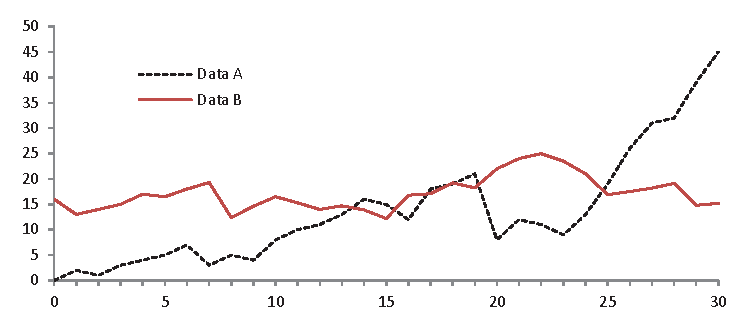
\includegraphics[width=\textwidth]{fig1.eps}
  \caption{A figure caption is always placed below the illustration.
    Please note that short captions are centered, while long ones are
  justified by the macro package automatically.} \label{fig1}
\end{figure}

Tabla~\ref{tab1} przedstawia że działa.

\begin{table}
  \caption{Table captions should be placed above the
  tables.}\label{tab1}
  \begin{tabular}{|l|l|l|}
    \hline
    Heading level &  Example & Font size and style\\
    \hline
    Title (centered) &  {\Large\bfseries Lecture Notes} & 14 point, bold\\
    1st-level heading &  {\large\bfseries 1 Introduction} & 12 point, bold\\
    2nd-level heading & {\bfseries 2.1 Printing Area} & 10 point, bold\\
    3rd-level heading & {\bfseries Run-in Heading in Bold.} Text follows & 10 point, bold\\
    4th-level heading & {\itshape Lowest Level Heading.} Text follows & 10 point, italic\\
    \hline
  \end{tabular}
\end{table}

% ########## END OF SAMPLES

\end{document}
